\chapter{ABLA V3 Evaporation with Fission}

\section{Introduction}

There is a renewed interest in the study of spallation reactions. This
is largely due to new technological applications, such as Accelerator
Driven Systems, consisting of sub-critical nuclear reactor and
particle accelerator. These applications require optimized spallation
targets or spallation sources. This type of problem has typically a large number
of parameters and thus it cannot be solved by trial and error
method. One has to rely on simulations, which implies that very
accurate simulation tools need to be developed and their validity and
accuracy needs also to be assessed.

Above the energy 200 MeV it is necessary to use reliable models due to
the prohibitive number of open channels. The most appropriate modeling
technique in this energy region is intranuclear cascade (INC) combined
with evaporation model. One such pair of models is the Li\`ege cascade
model INCL4.2 coupled with ABLA evaporation model. The strategy adopted
by the INCL4.2 cascade is to improve the quasi-classical treatment of
physics without relying on too many free parameters. 

This chapter introduces the physics provided by INCL4.2 and ABLA V3 codes as implemented in Geant4.
Tables \ref{tbl:inclsummary} and \ref{tbl:ablasummary} will summarize the key features 
and provides references describing in detail the physics.


\section{ABLA V3 evaporation}
\index{evaporation}

The ABLA V3 evaporation model takes excited nucleus parameters,
excitation energy, mass number, charge number and nucleus spin, as
input. It calculates the probabilities for emitting proton, neutron or
alpha particle and also probability for fission to occur. 
The summary of Geant4 ABLA V3 implementation is represented in Table \ref{tbl:ablasummary}.


The probabilities for emission of particle type $j$ are calculated using
formula:
\begin{equation}
W_j(N,Z,E) = \frac{\Gamma_j(N,Z,E)}{\sum_k\Gamma_k(N,Z,E)},
\label{eqn:probabilities}
\end{equation}
where $\Gamma_j$ is emission width for particle $j$, $N$ is neutron
number, $Z$ charge number and $E$ excitation energy. Possible emitted
particles are \emph{protons}, \emph{neutrons} and \emph{alphas}.
Emission widths are calculated using the following formula:
\index{emission width}
\begin{equation}
\Gamma_j = \frac{1}{2 \pi \rho_c(E)} \frac{4 m_j R^2}{\hbar^2} T_j^2 \rho_j(E - S_j - B_j),
\label{eqn:emissionwidth}
\end{equation}
where $\rho_c(E)$ and $\rho_j(E - S_j - B_j)$ are the level densities
of the compound nucleus and the exit channel, respectively. $B_j$ is
the height of the Coulomb barrier, $S_j$ the separation energy, $R$ is
the radius and $T_j$ the temperature of the remnant nucleus after
emission and $m_j$ the mass of the emitted particle.

The fission width is calculated from:
\index{fission width}
\begin{equation}
\Gamma_i = \frac{1}{2 \pi \rho_c(E)}T_f \rho_f(E - B_f),
\label{eqn:fissionwidth}
\end{equation}
where $\rho_f(E)$ is the level density of transition states in the
fissioning nucleus, $B_f$ the height of the fission barrier and $T_f$
the temperature of the nucleus.


\begin{table}[ht]
  \caption{ABLA V3 (located in the Geant4 directory
    {\tt source/\-processes/\-hadronic/\-models/\-incl}) feature summary.}
\label{tbl:ablasummary}
\vskip1cm
\begin{center}
\begin{tabular}{l|l}
\hline
{\bf Requirements} & \\
External data file & G4ABLA3.0 available at Geant4 site \\
Environment variable & {\tt G4ABLADATA} \\ 
for external data & \\
\hline
{\bf Usage}      & \\
Physics list     & Not yet implemented, \\
                 & instead use the interfaces directly. \\
\hline
{\bf Interfaces} &     \\
{\tt G4InclAblaCascadeInterface} &  h--A \\
{\tt G4InclAblaLightIonInterface} &  A--A \\
\hline
{\bf Supported input}     & Excited nuclei \\
\hline
{\bf Output particles}    & proton, neutron \\
                    & $\alpha$ \\
                    & fission products \\
                    & residual nuclei \\
\hline
{\bf Features} & evaporation of proton, neutron and $\alpha$ \\
                    & fission \\
\hline
{\bf Misc.}                & 5 classes, 5k lines \\
                    & 0.9 $<$ speed C++/F77 $<$ 1.1 \\
\hline
{\bf References}    & Key reference: \cite{Junghans98a}, see also \cite{Benlliure98a} \\
\hline
\end{tabular}
\end{center}
\end{table}

\subsection{Level densities}
\index{level density}

Nuclear level densities are calculated using the following formula:
\begin{equation}
  a = 0.073 A  [MeV^{-1}] + 0.095  B_s  A^{2/3} [MeV^{-2}],
\label{eqn:leveldensity}
\end{equation}
where $A$ the nucleus mass number and $B_s$ dimensionless surface area
of the nucleus. 

%The level density calculation is implemented in the
%code as follows:
%\begin{verbatim}
%pa = (ald->av)*a + (ald->as)*pow(a,(2.0/3.0)) 
%     + (ald->ak)*pow(a,(1.0/3.0));
%\end{verbatim}
%where {\tt ald->av} is 0.073, {\tt ald->as} is 0.095 and {\tt ald->ak}
%is 0.

\subsection{Fission}
\index{fission}

Fission barrier, used to calculate fission width
\ref{eqn:fissionwidth}, is calculated using a semi-empirical model
fitting to data obtained from nuclear physics experiments.


\section{External data file required}

Both INCL4.2 and ABLA V3 need data files. These files contain ABLA V3 shell corrections and remnant nucleus masses for INCL4.2. 
To enable this data set, environment variable {\tt G4ABLADATA} needs to be set, 
and the data downloaded from Geant4 web page. For Geant4 9.1 release use data file G4ABLA3.0

\section{Implementation details}
INCL4.2 and ABLA V3 are provided as alpha release for Geant4 9.1.
In this first release design follows as closely as possibly the original codes,
and class re-design is left for future Geant4 releases.
Current simple design is shown in  \ref{fig:uml}

\begin{figure}
\begin{center}
\includegraphics[angle=0,scale=1.0]{AblaUml.eps}
%\includegraphics[angle=0,scale=1,0]{hadronic/theory_driven/Incl/InclAblaUml.eps}
\end{center}
\caption[INCL4 and ABLA class diagram]{Simplified UML class diagram of
  INCL and ABLA implementations in Geant4.}
\label{fig:uml}
\end{figure}

Testing of INCL and ABLA models is based on ROOT \cite{Brun97a} scripting.

\section{Physics Performance}
INCL4.2 together with ABLA V3 provides an up to date modeling tool particularly for spallation
studies for hadron projectile energy range 200 MeV - 3 GeV. 
It provides an detailed description of double differential
energy spectrum of cascading particles (see \ref{fig:pPbDoubleDifferential}) and remnants.

Models are validated against recent data and continually updated.

\begin{figure}
\begin{center}
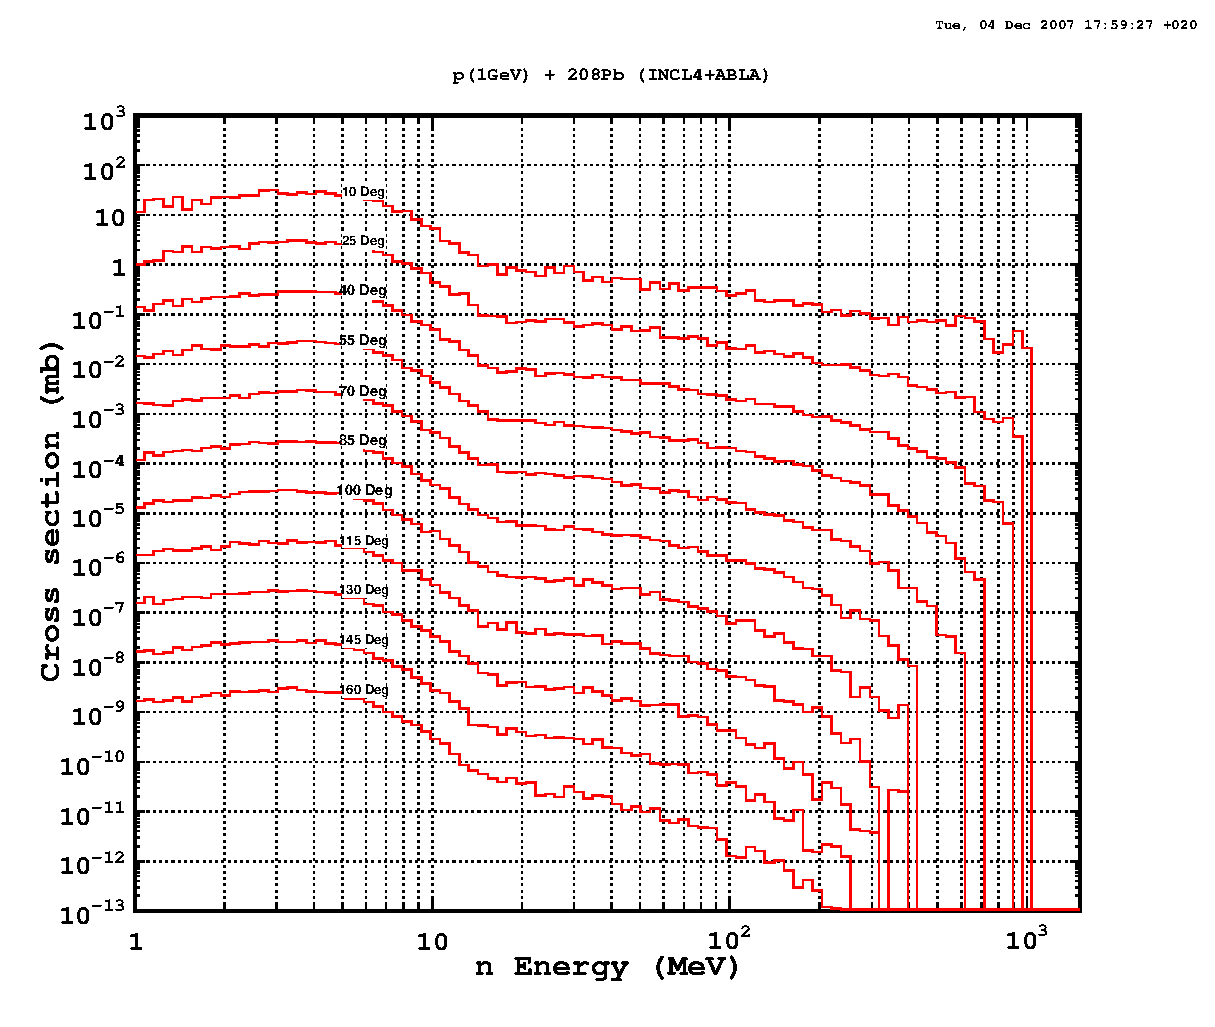
\includegraphics[angle=0,scale=0.65]{pPbDoubleDifferential.eps}
%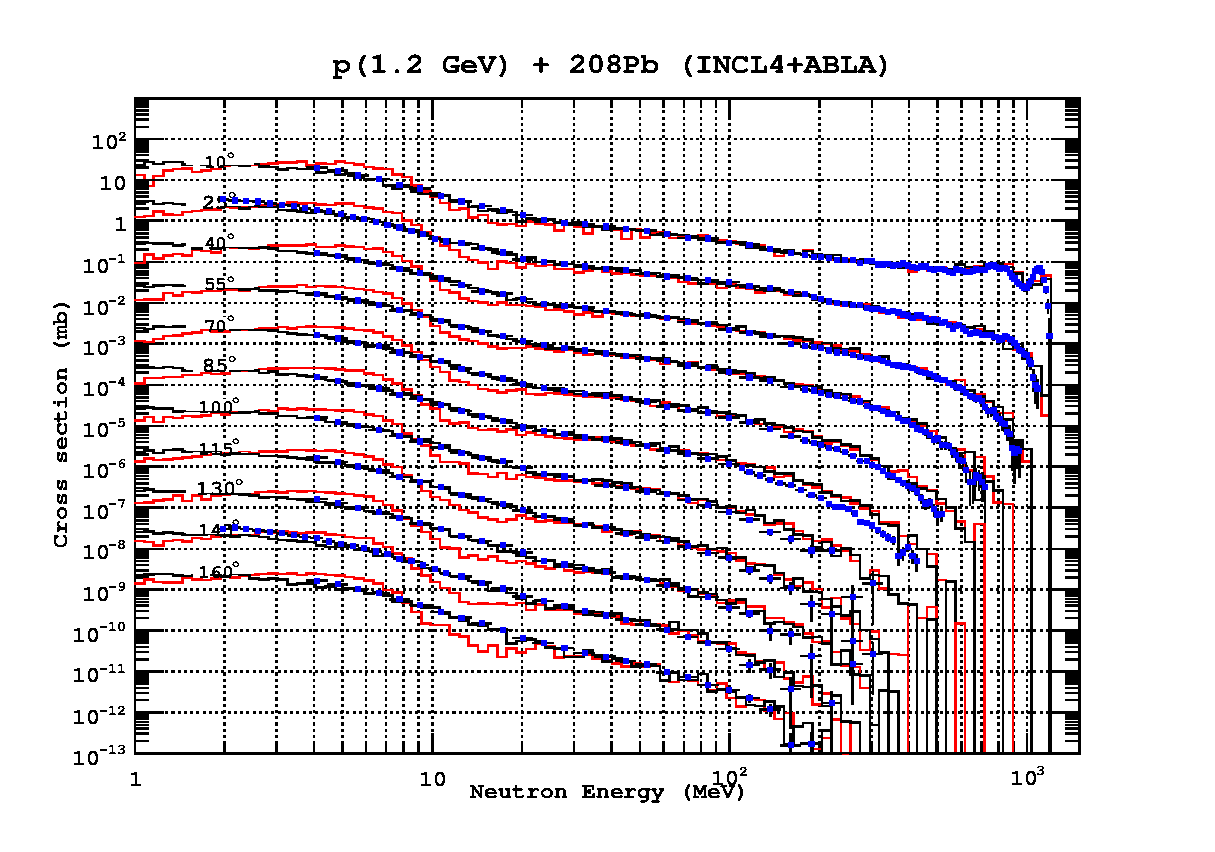
\includegraphics[angle=0,scale=0.6]{hadronic/theory_driven/Incl/pPbDoubleDifferential.eps}
\end{center}
\caption{Geant4 implementation of INCL4.2 together with ABLA V3. Neutron double differential cross sections of reaction p(1GeV) + Pb
 For more detailed discussion on this subject
%  double differential cross sections for proton-induced reactions on
%  Pb targets with comparison to experimental data 
see reference \cite{Boudard02a}.}
\label{fig:pPbDoubleDifferential}
\end{figure}

\section{Status of this document}

{\bf 06.12.2007} Documentation for alpha release added. Pekka
Kaitaniemi, HIP (translation); Alain Boudard, CEA (contact person
INCL/ABLA); Joseph Cugnon, University of Li\`ege (INCL physics
modelling); Karl-Heintz Schmidt, GSI (ABLA); Christelle Schmidt, IPNL
(fission code); Aatos Heikkinen, HIP (project coordination)

% \begin{thebibliography}{99}
% \bibitem{incl1} J. Cugnon et al \emph{Nuc. Phys. A352} (1981) 505
% \bibitem{incl2} J. Cugnon et al \emph{Nuc. Phys. A462} (1987) 751
% \bibitem{incl3} J. Cugnon et al \emph{Nuc. Phys. A500} (1989) 701
% \bibitem{incl4} A. Boudard et al \emph{Phys. Rev. C66} (2002) 044615
% \bibitem{liegeuniversity} Li\`ege University
% \href{http://www.ulg.ac.be/foreign/}{{\tt http://www.ulg.ac.be/foreign/}}
% \bibitem{cea} CEA website
%   \href{http://www.cea.fr/gb/index.asp}{{\tt http://www.cea.fr/gb/index.asp}}
% \end{thebibliography}

\begin{thebibliography}{99}

% \bibitem{alsmiller90}
%   R.G. Alsmiller and F.S. Alsmiller and O.W. Hermann,
%   The high-energy transport code HETC88 and comparisons with experimental data,
%   Nuclear Instruments and Methods in Physics Research A 295,
%    (1990), 337--343,

% [1] Barashenkov V.S., Toneev V.D. High Energy interactions of particles and nuclei with nuclei. Moscow, 1972 
%(in Russian, but there is an English translation)) 

\bibitem{Boudard02a} A. Boudard et al \emph{Phys. Rev. C66} (2002) 044615
\bibitem{Cugnon81a} J. Cugnon et al \emph{Nuc. Phys. A352} (1981) 505
\bibitem{Cugnon87a} J. Cugnon et al \emph{Nuc. Phys. A462} (1987) 751
\bibitem{Cugnon89a} J. Cugnon et al \emph{Nuc. Phys. A500} (1989) 701
\bibitem{Cugnon97a} J. Cugnon et al \emph{Nuc. Phys. A620} (1997) 745
\bibitem{Junghans98a} A.R. Junghans et al \emph{Nuc. Phys. A629} (1998) 635
\bibitem{Benlliure98a} J. Benlliure et al \emph{Nuc. Phys. A628} (1998) 458
\bibitem{Kaitaniemi07a} P. Kaitaniemi et al. \emph{Implementation of
    INCL4 cascade and ABLA evaporation codes in Geant4} (To be
    published in the proceedings of CHEP 2007, September 2-6,
    Victoria, BC, Canada.)
\bibitem{Brun97a} R. Brun, F. Rademakers \emph{Nucl. Inst \&
    Meth. in Phys. Res. A 389} (1997) 81
\end{thebibliography}
